\documentclass[11pt]{article}

\usepackage[a4paper,margin=27mm]{geometry}
\usepackage{amsmath,amssymb,mathtools}
\usepackage{booktabs,array}
\usepackage{graphicx}
\usepackage{xcolor}
\usepackage{microtype}
\usepackage{hyperref}
\usepackage{natbib}

\hypersetup{
  colorlinks=true,
  linkcolor=blue!45!black,
  citecolor=blue!45!black,
  urlcolor=blue!55!black,
  pdftitle={Monetary--Fiscal Coordination as a State-Contingent Dynamic Game}
}
\graphicspath{{output/}}
\setlength{\parskip}{0.45em}
\setlength{\parindent}{1.3em}
\setlength{\emergencystretch}{2em}
\newcommand{\E}{\mathbb{E}}
\newcommand{\R}{\mathbb{R}}
\newcommand{\loss}{\mathcal{L}}
\newcolumntype{P}[1]{>{\raggedright\arraybackslash}p{#1}}

\title{Monetary--Fiscal Coordination as a State-Contingent Dynamic Game:\\
Steady States, Shocks, Commitment, and an Australian Calibration}
\author{Matt Nolan \and Gulnara Nolan \and Vladimir Petkov}
\date{Research draft --- \today}

\begin{document}
\maketitle

\begin{abstract}
This paper develops a monetary--fiscal policy game calibrated to Australian
data.  It keeps a single social-welfare criterion fixed while allowing the
central bank and fiscal authority to place different relative weights on
inflation and the output gap.  We first solve cooperative, simultaneous Nash,
and Stackelberg versions of a finite-horizon open-loop game.  With no shock and
zero gap targets, every solution has the same zero steady state; demand and
cost-push shocks activate large policy-mix externalities.  We then solve a
recursive linear--quadratic game in which output, inflation, debt, and lagged
instruments are states, and policies are stationary Markov feedback rules.
Adjustment costs make current instruments investments in future strategic
positions.  In a first institutional stage, each authority delegates an
adjustment coefficient to its future policymaker; in the second stage, the
policymakers play the feedback Nash game after shocks.  The Australian feedback
equilibrium is stable and strongly history dependent.  The institutional Nash
choice, $(\lambda_M,\lambda_F)=(0.05,0.04)$, equals the primitive adjustment
weights, while the social design is $(0.05,0.115)$.  Thus the baseline does not
manufacture a commitment arms race: it shows under-provision of fiscal inertia.
Recursive Nash raises social loss by only 0.49 per cent after a demand shock and
0.06 per cent after a cost-push shock, much less than the open-loop benchmark.
The difference is economically informative but not a clean horse race because
the recursive implementation uses an estimated semi-structural timing closure.
Open-loop commitment, Markov discretion, and institutional design answer
different questions and should be reported separately.
\end{abstract}

\noindent\textbf{Keywords:} monetary--fiscal coordination; dynamic games;\\
Markov-perfect equilibrium; strategic complementarity; fiscal dominance;
Australia.\\
\textbf{JEL codes:} E52, E58, E61, E62, C73.

\section{Introduction}

Monetary and fiscal authorities act on the same economy but need not evaluate
the resulting inflation, activity, debt, or instrument movements in the same
way.  This observation is enough to create a policy game even when both
institutions are benevolent and the model contains no political distortion.
It does not, however, imply that every shock produces the same kind of game.
Whether the instruments are strategic complements or substitutes, whether an
authority free rides, and whether leadership improves outcomes depend on the
shock, nominal rigidity, the state variables, and the timing of commitment.

The motivating draft distinguishes two mechanisms.  Following a demand shock,
both authorities want to stabilise activity but may try to shift the adjustment
cost to the other authority---a ``GFC effect.''  Following a supply disturbance,
the central bank's concern for inflation can produce tightening while the
fiscal authority's concern for activity produces expansion.  The policies then
offset one another at the macroeconomic level while becoming mutually
reinforcing in their numerical instrument settings---a ``post-COVID effect.''
The draft also makes prior policy a state through adjustment costs and asks
whether institutions deliberately acquire commitment technology.  These are
recursive, state-contingent questions.

The first computational block answers a narrower but useful question.  At the
beginning of a finite horizon, after a shock path is known, the authorities
choose complete instrument paths.  This open-loop game isolates the policy-mix
externality and provides a benchmark.  The new recursive block instead lets
authorities reoptimise at every observed state and makes today's instruments
tomorrow's lagged-policy states.  A first-stage institutional game then lets
each authority choose the adjustment coefficient delegated to its future self.

This revision makes that boundary explicit.  It contributes five results.
First, it embeds fiscal policy and debt in a transparent extension of the
three-equation New Keynesian model.  Second, it separates agency mandates from
true social welfare.  Third, it establishes experimentally that the calibrated
no-shock steady state contains no realised conflict, while shocks generate
large policy-game losses in the open-loop benchmark.  Fourth, it solves the
recursive Markov-perfect game requested in the original draft.  Fifth, it
solves a two-stage institutional game in delegated adjustment costs and shows
that, at the Australian baseline, decentralised authorities retain their
primitive inertia while a social designer chooses substantially more fiscal
inertia.  Open-loop Nash and leadership remain benchmarks rather than final
equilibrium concepts.

\section{From three equations to a monetary--fiscal game}

\subsection{The private-economy block}

Let $x_t$ denote the output gap, $\pi_t$ inflation relative to target, $i_t$
the monetary-policy instrument relative to neutral, and $g_t$ a fiscal-demand
instrument, where $g_t>0$ is expansionary.  A compact forward-looking model is
\begin{align}
 x_t &= \E_t x_{t+1}
       - \sigma\bigl(i_t-\E_t\pi_{t+1}\bigr)
       + \psi g_t + d_t,                                      \label{eq:is}\\
 \pi_t &= \beta\E_t\pi_{t+1}+\kappa x_t+u_t,                  \label{eq:pc}\\
 b_{t+1} &= \rho_b b_t+\chi_g g_t+\chi_i i_t-\chi_\pi\pi_t . \label{eq:debt}
\end{align}
Here $d_t$ is a demand disturbance, $u_t$ is a cost-push disturbance, and
$b_t$ is the public-debt gap.  The signs match the code: a larger $i_t$ is
tighter and a larger $g_t$ is more expansionary.  Equation \eqref{eq:is} is the
IS curve, \eqref{eq:pc} is the New Keynesian Phillips curve, and
\eqref{eq:debt} is a deliberately parsimonious debt law.

It is potentially misleading to call this merely a ``four-equation model.''
The conventional three-equation model consists of IS, Phillips, and an
exogenous monetary rule.  Once both policies are optimised, the Taylor rule is
replaced by the central bank's first-order condition and a fiscal first-order
condition is added.  With debt retained, the equilibrium has five blocks:
IS, Phillips, debt accumulation, monetary optimality, and fiscal optimality.
For active--passive regime comparisons we also use the explicit rule closure
\begin{align}
 i_t &= \rho_i i_{t-1}+(1-\rho_i)(\phi_\pi\pi_t+\phi_xx_t)+\varepsilon^i_t,
                                                                  \label{eq:mrule}\\
 g_t &= \rho_g g_{t-1}-(1-\rho_g)(\gamma_bb_t+\gamma_xx_t)+\varepsilon^g_t.
                                                                  \label{eq:frule}
\end{align}
Equations \eqref{eq:mrule}--\eqref{eq:frule} are an alternative closure, not
additional behavioural assumptions inside the optimising game.

\subsection{One social objective, two agency mandates}

The primitive social loss is fixed across every game:
\begin{align}
 \loss^S = \frac12\E_0\sum_{t=0}^{\infty}\beta^t\bigl[
 &\omega_\pi^S\pi_t^2+\omega_x^Sx_t^2+\omega_b^Sb_t^2
 +\omega_i^Si_t^2+\omega_g^Sg_t^2 \notag\\
 &+\omega_{\Delta i}^S(i_t-i_{t-1})^2
 +\omega_{\Delta g}^S(g_t-g_{t-1})^2\bigr].                 \label{eq:social}
\end{align}
It is the welfare yardstick and therefore does not change when the strategic
regime changes.  Cooperation means that a single planner minimises
\eqref{eq:social}; it does not mean adding together two differently weighted
agency losses.

The agency losses have the same form but different inflation and output-gap
weights:
\begin{equation}
 \loss^j=\frac12\E_0\sum_{t=0}^{\infty}\beta^t
 \left[\omega_\pi^j\pi_t^2+\omega_x^jx_t^2+
 \omega_b b_t^2+\omega_i i_t^2+\omega_g g_t^2+
 \omega_{\Delta i}(\Delta i_t)^2+
 \omega_{\Delta g}(\Delta g_t)^2\right],                    \label{eq:agency}
\end{equation}
where $j\in\{M,F\}$.  In the baseline calibration the monetary authority is
more inflation averse, $(\omega_\pi^M,\omega_x^M)=(1.5,0.25)$, while the fiscal
authority is more output oriented,
$(\omega_\pi^F,\omega_x^F)=(0.5,0.75)$.  All other weights are held fixed.
The social weights are $(\omega_\pi^S,\omega_x^S)=(1,0.5)$.  Thus the
experiment changes mandates, not technology or the definition of welfare.

This distinction also explains why cooperation can involve a larger response
by one instrument than a decentralised equilibrium.  Cooperation internalises
both instruments' effects and assigns the policy mix according to
\eqref{eq:social}.  Nash policymakers instead minimise different losses and may
partially offset or free ride on one another.  A larger cooperative movement is
not generated by changing the planner's weights across cases; it is an
equilibrium allocation of a fixed social objective.

\section{Timing, states, and equilibrium concepts}

\subsection{Shocks and the strategic state}

For the intended stochastic model, take
\begin{align}
 d_{t+1}&=\rho_d d_t+\varepsilon^d_{t+1}, &
 u_{t+1}&=\rho_u u_t+\varepsilon^u_{t+1},                       \label{eq:shocks}
\end{align}
with innovations not known at $t$.  The implemented recursive state is
\begin{equation}
 z_t=(x_{t-1},\pi_{t-1},b_t,i_{t-1},g_{t-1},d_t,u_t)' .          \label{eq:state}
\end{equation}
Lagged instruments matter because adjustment costs make past policy affect the
current marginal cost of action.  Debt transmits fiscal and monetary choices
across time.  Persistent shocks change the distribution of future states.
Lagged output and inflation implement the Australian semi-structural timing
closure described below.  A fully forward-looking New Keynesian implementation
would instead augment the state with equilibrium expectational variables and,
under Ramsey commitment, promised inflation or planner multipliers.

The timeline is: the state $z_t$ is observed; private agents form rational
expectations using anticipated policy functions; the authorities choose their
instruments according to the equilibrium timing; outcomes occur; and new
innovations produce $z_{t+1}$.  This timing makes the policies contingent on
the realised state, not just on calendar time.

\subsection{Feedback Nash and Markov perfection}

Let the strategy functions be
\begin{equation}
 i_t=F_M(z_t),\qquad g_t=F_F(z_t).                               \label{eq:feedback}
\end{equation}
A stationary Markov-perfect Nash equilibrium is a pair $(F_M,F_F)$ such that,
given the other authority's policy function and rational private expectations,
each authority solves its Bellman problem at every state.  Schematically,
\begin{align}
 V_M(z)&=\min_i\left\{\ell_M(z,i,F_F(z))+
          \beta\E[V_M(z')\mid z,i,F_F(z)]\right\},             \label{eq:bellmanM}\\
 V_F(z)&=\min_g\left\{\ell_F(z,F_M(z),g)+
          \beta\E[V_F(z')\mid z,F_M(z),g]\right\}.             \label{eq:bellmanF}
\end{align}
In the linear--quadratic approximation, value functions are quadratic and the
policy functions are linear, $i_t=-K_Mz_t$ and $g_t=-K_Fz_t$.  The equilibrium
is obtained from coupled Riccati equations, with stabilising and determinacy
conditions imposed on the joint private-policy system.

To see the investment channel, write the recursive transition as
$z'=Az+B_Mi+B_Fg$.  Given quadratic continuation matrices $P_M$ and $P_F$, the
simultaneous policy first-order conditions have the form
\begin{equation}
 \begin{bmatrix}
  Q^M_{ii}+\beta B_M'P_MB_M & Q^M_{ig}+\beta B_M'P_MB_F\\
  Q^F_{gi}+\beta B_F'P_FB_M & Q^F_{gg}+\beta B_F'P_FB_F
 \end{bmatrix}
 \begin{bmatrix}i_t\\g_t\end{bmatrix}
 =-
 \begin{bmatrix}
  Q^M_{iz}+\beta B_M'P_MA\\
  Q^F_{gz}+\beta B_F'P_FA
 \end{bmatrix}z_t .                                             \label{eq:feedback-foc}
\end{equation}
The vectors $B_M$ and $B_F$ contain unit loadings that make $i_t$ and $g_t$
next period's lagged instruments.  Hence the continuation terms in
\eqref{eq:feedback-foc} are the formal strategic-investment motive: a current
instrument changes future macro states, future adjustment costs, and the other
authority's future feedback action.

This is the natural main solution concept for the original draft.  The
authority that deviates today understands how the deviation changes debt and
the next period's adjustment-cost state, but it cannot bind its future self to
ignore information that will later be available.  Consequently the solution
speaks directly to credibility, reoptimisation, and policy used as a strategic
state.

\subsection{What open-loop equilibrium does and does not mean}

The open-loop numerical block instead selects complete paths
$I=(i_0,\ldots,i_{T-1})'$ and $G=(g_0,\ldots,g_{T-1})'$ at date zero.  Conditional
on a known shock path, the linear economy can be written
\begin{equation}
 q=q^0+A_I I+A_GG,                                               \label{eq:pathmap}
\end{equation}
where $q$ stacks macroeconomic outcomes.  Quadratic agency losses imply affine
best responses
\begin{equation}
 I=a_M+B_MG,\qquad G=a_F+B_FI.                                  \label{eq:br}
\end{equation}
The open-loop Nash path solves the two equations simultaneously.  The
round-trip matrix $B_MB_F$ measures the strength of iterative reaction, and
$\rho(B_MB_F)<1$ is a useful local convergence diagnostic.

Open-loop equilibrium is appropriate if the economic experiment is explicitly
one of full path commitment after the shock is observed and no unanticipated
innovation subsequently arrives.  It is also valuable as a transparent
benchmark.  It is not sufficient when the object of interest is policy under
recurring shocks, discretion, or strategic investment in adjustment costs.
The path is time-indexed rather than state-contingent, and an authority does not
reoptimise after histories that were not anticipated at date zero.

Nor does the spectral radius alone identify strategic complementarity.  It is
unsigned and summarises a high-dimensional round trip.  Classification requires
the signed cross-derivatives $\partial i_t/\partial g_s$ and
$\partial g_t/\partial i_s$, evaluated at an economically specified state or
shock.  With the present sign convention, positive contemporaneous slopes are
complementarity in instrument levels: fiscal expansion elicits monetary
tightening, and tighter money elicits more fiscal expansion.  The two policies
then offset one another in aggregate demand.

\subsection{Leadership and the commitment meta-game}

The existing Stackelberg calculations are also open loop.  A leader chooses a
complete path while internalising the follower's complete-path best response.
This can make monetary and fiscal leadership look similar because both leaders
have nearly the same ability to exploit the same linear reaction mapping and
because the calibration is close to a common welfare problem once the follower
is internalised.

The recursive counterpart is feedback Stackelberg equilibrium.  There the
leader anticipates the follower's state-contingent response at every future
state.  The original draft additionally suggests a prior institutional stage:
before shocks are realised, authorities choose commitment or adjustment-cost
parameters, say $\lambda_M$ and $\lambda_F$; after shocks, they play the
feedback policy game.  Formally, the ex ante problem is
\begin{equation}
 \lambda_j^*\in\arg\min_{\lambda_j}\;
 \E\!\left[V_j\bigl(z_0;\lambda_j,\lambda_{-j}\bigr)\right],     \label{eq:meta}
\end{equation}
where $V_j$ is generated by the continuation MPE.  In the implementation, the
delegated coefficient replaces the own-instrument adjustment coefficient in
the future policymaker's operational problem, but the stage-one authority
evaluates the outcome using its original mandate.  Its institutional objective
is
\begin{equation}
 \mathcal J_j(\lambda_j,\lambda_{-j})=
 \E\loss^j_{\mathrm{primitive}}\!\left(F_M(\lambda),F_F(\lambda)\right)
 +c_\lambda(\lambda_j-\bar\lambda_j)^2,                         \label{eq:investment}
\end{equation}
where $\bar\lambda_j$ is the primitive adjustment weight.  Centering the
implementation cost at the primitive separates strategic delegation from an
arbitrary mechanical preference for zero inertia.  A constitutional planner
chooses both coefficients using \eqref{eq:social} and the sum of implementation
costs.  This separates leadership within stabilisation from the acquisition of
commitment technology.

\section{The steady state and the shock-contingent type of game}

\subsection{No-shock steady state}

Set $d=u=0$ and use zero gap targets.  Equations
\eqref{eq:is}--\eqref{eq:debt} and either policy closure admit
\begin{equation}
 x^*=\pi^*=b^*=i^*=g^*=0.                                      \label{eq:ss}
\end{equation}
Every term in each quadratic loss is then zero.  Because policy costs are
strictly convex, no authority can improve on this allocation by moving its
instrument.  The numerical zero-shock experiment verifies that cooperation,
Nash, monetary leadership, and fiscal leadership all return exactly this
steady state.

This finding should be stated carefully.  It does not say that institutions or
coordination are irrelevant in normal times.  Reaction slopes and the welfare
consequences of future states remain latent, and an ex ante commitment choice
can still matter because shocks occur with positive probability.  It says that
the present aligned-target calibration does not generate a realised
steady-state policy conflict.  A non-zero steady-state game would require an
additional wedge such as different inflation targets, a fiscal spending bias,
distortionary tax objectives, a debt target conflict, or seigniorage pressure.

\begin{table}[htbp]
\centering
\caption{Numerical no-shock steady state}
\label{tab:ss}
\begin{tabular}{lccccc}
\toprule
Strategy & social loss & $\max|x|$ & $\max|\pi|$ & $\max|i|$ & $\max|g|$\\
\midrule
Cooperation       & 0 & 0 & 0 & 0 & 0\\
Simultaneous Nash & 0 & 0 & 0 & 0 & 0\\
Monetary leader   & 0 & 0 & 0 & 0 & 0\\
Fiscal leader     & 0 & 0 & 0 & 0 & 0\\
\bottomrule
\end{tabular}
\end{table}

\subsection{A taxonomy by shock}

The shock determines which disagreement is economically active.  Table
\ref{tab:taxonomy} gives the disciplined interpretation intended for the full
feedback model.

\begin{table}[htbp]
\centering
\caption{Shock-contingent strategic interaction}
\label{tab:taxonomy}
\small
\begin{tabular}{P{0.17\textwidth}P{0.235\textwidth}P{0.245\textwidth}P{0.24\textwidth}}
\toprule
State & Main policy trade-off & Likely strategic mechanism & Empirical diagnostic\\
\midrule
No shock, aligned targets & None realised at the zero-gap steady state
& Dormant reaction structure; coordination matters ex ante
& Identical zero policies and losses\\
Demand contraction & Both agencies favour expansion, but dislike changing
their own instruments & Burden sharing and free riding; stabilisation efforts
can be substitutes & Signed cross-responses and each authority's contribution
to closing the output gap\\
Cost-push inflation & Inflation stabilisation conflicts with output
stabilisation & Monetary tightening and fiscal expansion can be complements in
instrument levels but offsets in demand & Signed policy slopes, policy-mix
distance, inflation/output outcomes\\
Debt or solvency shock & Price stability, debt stabilisation, and valuation
effects interact & Active--passive regimes and possible fiscal dominance
& Determinacy, debt backing, and nominal-liability valuation\\
\bottomrule
\end{tabular}
\end{table}

Nominal rigidity is pivotal after a cost-push shock.  When $\kappa$ is finite,
lower inflation requires an output sacrifice.  Because the monetary authority
places greater weight on inflation and the fiscal authority places greater
weight on output, their preferred points on that trade-off differ.  The fiscal
response then raises the central bank's desired rate, while the monetary
response raises the fiscal authority's desired support.  This is precisely the
case in which feedback, expectations, and commitment may alter the result most.

\section{Australian calibration and computation}

The code is written entirely in Julia.  The descriptive IS and Phillips
coefficients are estimated using quarterly Australian data over 1993Q1--2019Q4,
with public series cached alongside checksums for reproducibility.  The sample
ends before the pandemic so that the cost-push experiment is not mechanically
fit to the episode it is intended to illuminate.  The debt block and welfare
weights are transparent calibrations rather than claimed structural estimates.

The open-loop benchmark retains equations \eqref{eq:is}--\eqref{eq:debt}.  The
recursive experiment uses the directly estimable semi-structural timing
\begin{align}
 x_t &= \rho_xx_{t-1}-\sigma(i_t-\pi_{t-1})+\psi g_t+d_t,       \label{eq:ris}\\
 \pi_t &= \rho_\pi\pi_{t-1}+\kappa x_t+u_t,                    \label{eq:rpc}\\
 b_{t+1} &= \rho_bb_t+\chi_gg_t+\chi_ii_t-\chi_\pi\pi_t.       \label{eq:rdebt}
\end{align}
Current shocks are observed before policy.  The controls affect current output,
output affects current inflation, and current inflation affects end-of-period
debt.  Equations \eqref{eq:ris}--\eqref{eq:rdebt}, lagged instruments, and
shock laws form a linear transition $z_{t+1}=Az_t+B_Mi_t+B_Fg_t+\varepsilon_{t+1}$.
This closure is recursive and empirically transparent, but it is not identical
to the forward-looking private-sector block; the two sets of welfare numbers
must therefore not be interpreted as a controlled comparison of solution
concepts alone.

\begin{table}[htbp]
\centering
\caption{Selected baseline parameters}
\label{tab:calibration}
\begin{tabular}{lll}
\toprule
Parameter & Value & Interpretation\\
\midrule
$\beta$ & 0.9900 & quarterly discount factor\\
$\sigma$ & 0.03695 & semi-elasticity to the real-rate gap\\
$\psi$ & 0.05142 & public-demand multiplier in the IS equation\\
$\kappa$ & 0.15511 & Phillips-curve slope\\
$\rho_x$ & 0.62875 & output-gap persistence in recursive model\\
$\rho_\pi$ & 0.56255 & inflation persistence in recursive model\\
$\rho_b$ & 0.995 & debt persistence\\
$(\omega_\pi^S,\omega_x^S,\omega_b^S)$ & $(1,0.5,0.15)$ & social weights\\
$(\omega_\pi^M,\omega_x^M)$ & $(1.5,0.25)$ & monetary mandate\\
$(\omega_\pi^F,\omega_x^F)$ & $(0.5,0.75)$ & fiscal mandate\\
\bottomrule
\end{tabular}
\end{table}

For each deterministic shock path, the program constructs the linear path map
\eqref{eq:pathmap}, derives exact quadratic best responses, and solves four
regimes: the social planner, simultaneous Nash, monetary leadership, and fiscal
leadership.  It also varies mandate divergence and policy adjustment costs,
and solves the explicit rule system in monetary- and fiscal-dominance analogues.
For the recursive experiment, coupled algebraic Riccati iterations solve the
feedback Nash value functions.  A grid over delegated adjustment coefficients
$[0,0.15]^2$ with spacing 0.005 solves the first-stage game; the implementation
cost is $c_\lambda=0.005$.

\begin{figure}[htbp]
\centering
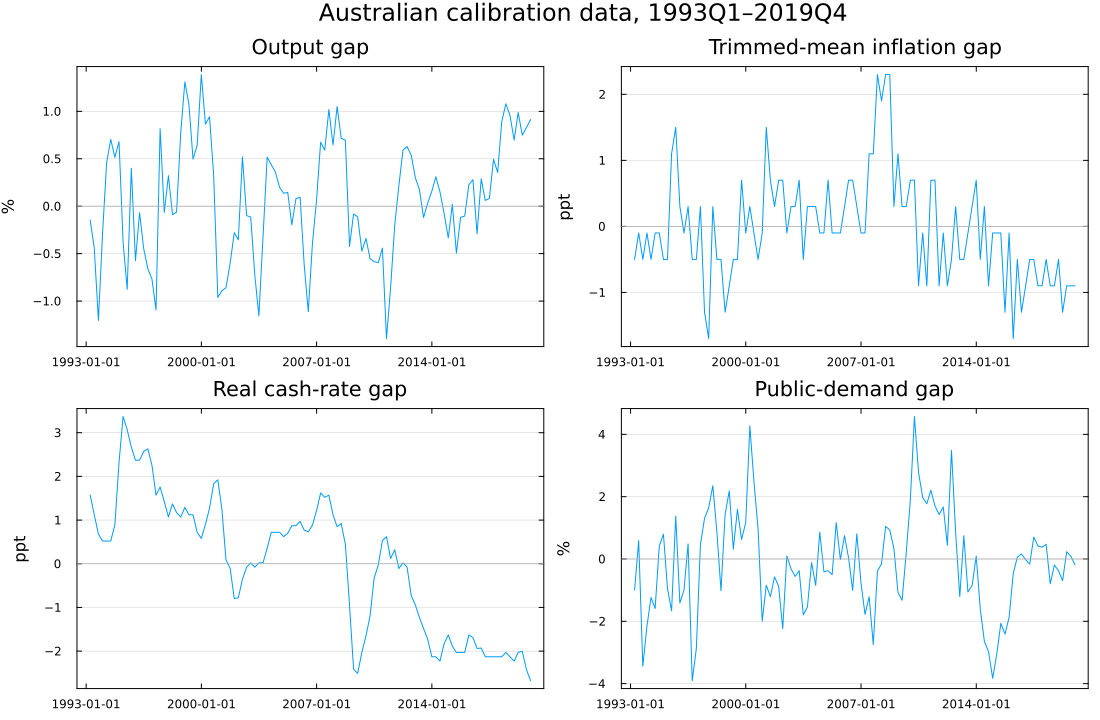
\includegraphics[width=0.92\textwidth]{australian_calibration_data.png}
\caption{Australian data used for the descriptive calibration.}
\label{fig:data}
\end{figure}

\section{Results}

\subsection{Shocks activate the coordination problem}

Figure \ref{fig:activation} scales the demand and cost-push innovations from
zero to 1.5 sample standard deviations.  At zero, the Nash welfare gap and the
distance between cooperative and Nash policy paths are both zero.  As shocks
grow, the path distance rises linearly and excess Nash loss rises quadratically,
as expected in a linear--quadratic model.  The supply-shock curves are steeper:
the shock activates the disagreement over the inflation--output trade-off.

\begin{figure}[htbp]
\centering
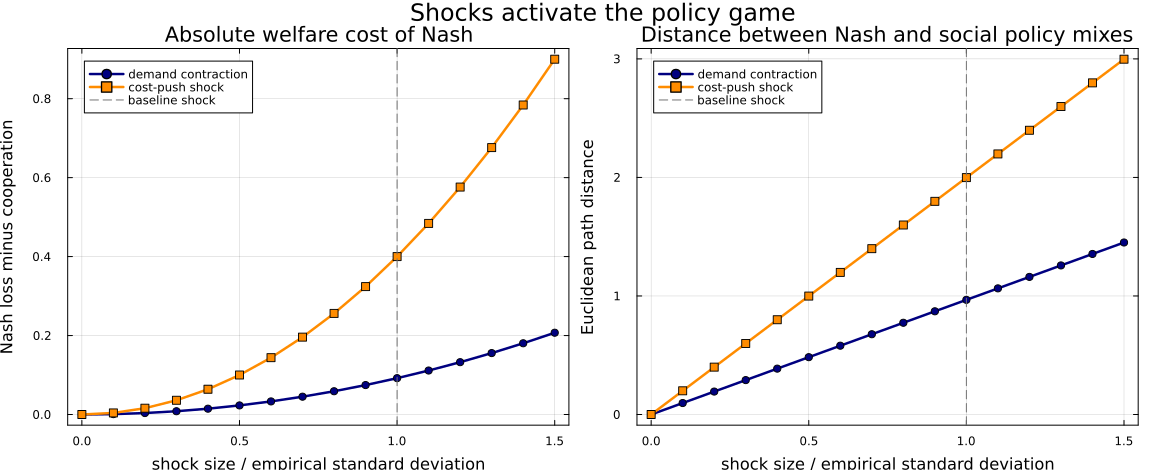
\includegraphics[width=0.94\textwidth]{shock_activation.png}
\caption{Shock activation of the coordination problem.  The left panel is
$\loss^S_{N}-\loss^S_{C}$; the right panel is the Euclidean distance between
the Nash and cooperative instrument paths.}
\label{fig:activation}
\end{figure}

\subsection{Demand contraction: burden sharing and free riding}

After a one-standard-deviation contractionary demand shock, cooperative social
loss is 0.0972 and simultaneous Nash loss is 0.1892, a 94.8 per cent increase.
The peak monetary response is 0.067 under cooperation but 0.306 under Nash;
the peak fiscal response is 0.075 under cooperation and 0.257 under Nash.  The
large gross movements do not indicate stronger stabilisation.  They partly
reflect the authorities reacting to and offsetting the policy mix generated by
the other authority.  The output peaks remain similar, while debt accumulation
is much larger under Nash.

The open-loop leadership outcomes are close to the planner: social loss is
0.0991 with monetary leadership and 0.0986 with fiscal leadership.  This result
shows that internalising the follower's reaction removes most of the static
path externality.  It should not yet be read as evidence that the institutional
identity of the leader is unimportant.  Feedback leadership may differ because
debt and lagged instruments change subsequent bargaining positions, while an
ex ante commitment choice changes continuation values before the shock occurs.

\begin{figure}[htbp]
\centering
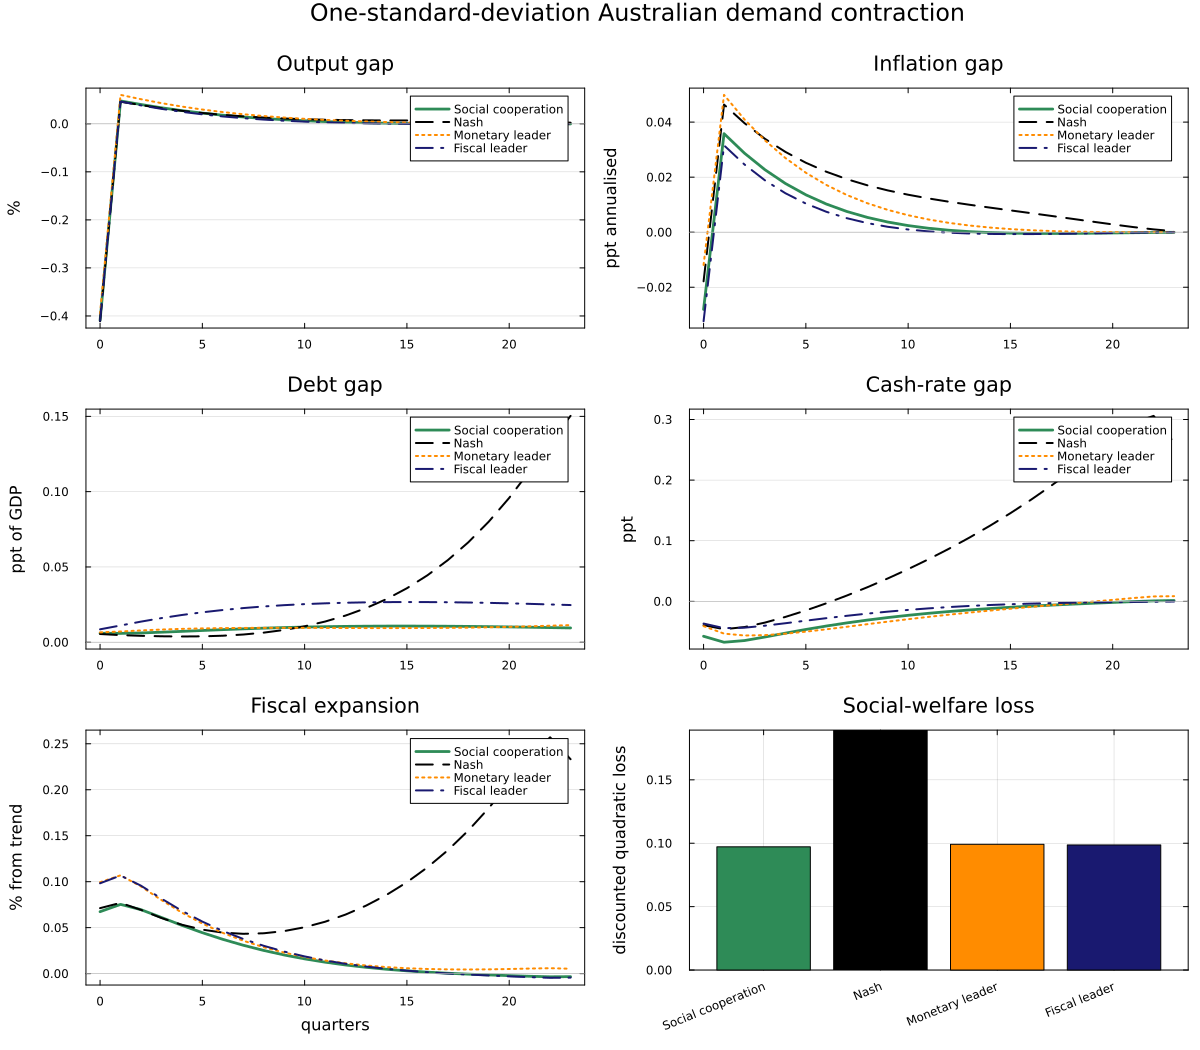
\includegraphics[width=0.94\textwidth]{demand_shock_game.png}
\caption{Responses to a contractionary demand shock under cooperation,
simultaneous open-loop Nash, and open-loop leadership.}
\label{fig:demand}
\end{figure}

\subsection{Cost-push shock: the offsetting-policy game}

After a one-standard-deviation cost-push shock, cooperative social loss is
0.3762 and Nash loss is 0.7762, an increase of 106.3 per cent.  Nash produces a
peak monetary response of 0.607 and a peak fiscal response of 0.500, compared
with 0.050 and 0.046 under cooperation.  This is the clearest baseline example
of strategic complementarity in instrument levels.  The central bank tightens
against inflation; the fiscal authority supports activity; each action raises
the other's incentive to respond.  Because $i_t$ and $g_t$ enter the IS curve
with opposite signs, complementarity between the numerical instruments means
macroeconomic offset, not common-direction stimulus.

Again, open-loop leadership nearly restores cooperative welfare: social loss
is about 0.386 under either leader.  The similarity follows from the common
linear path technology and the leader's internalisation of the follower's
full-path response.  Whether it survives recursive reoptimisation is a
substantive question for the feedback Stackelberg experiment.

\begin{figure}[htbp]
\centering
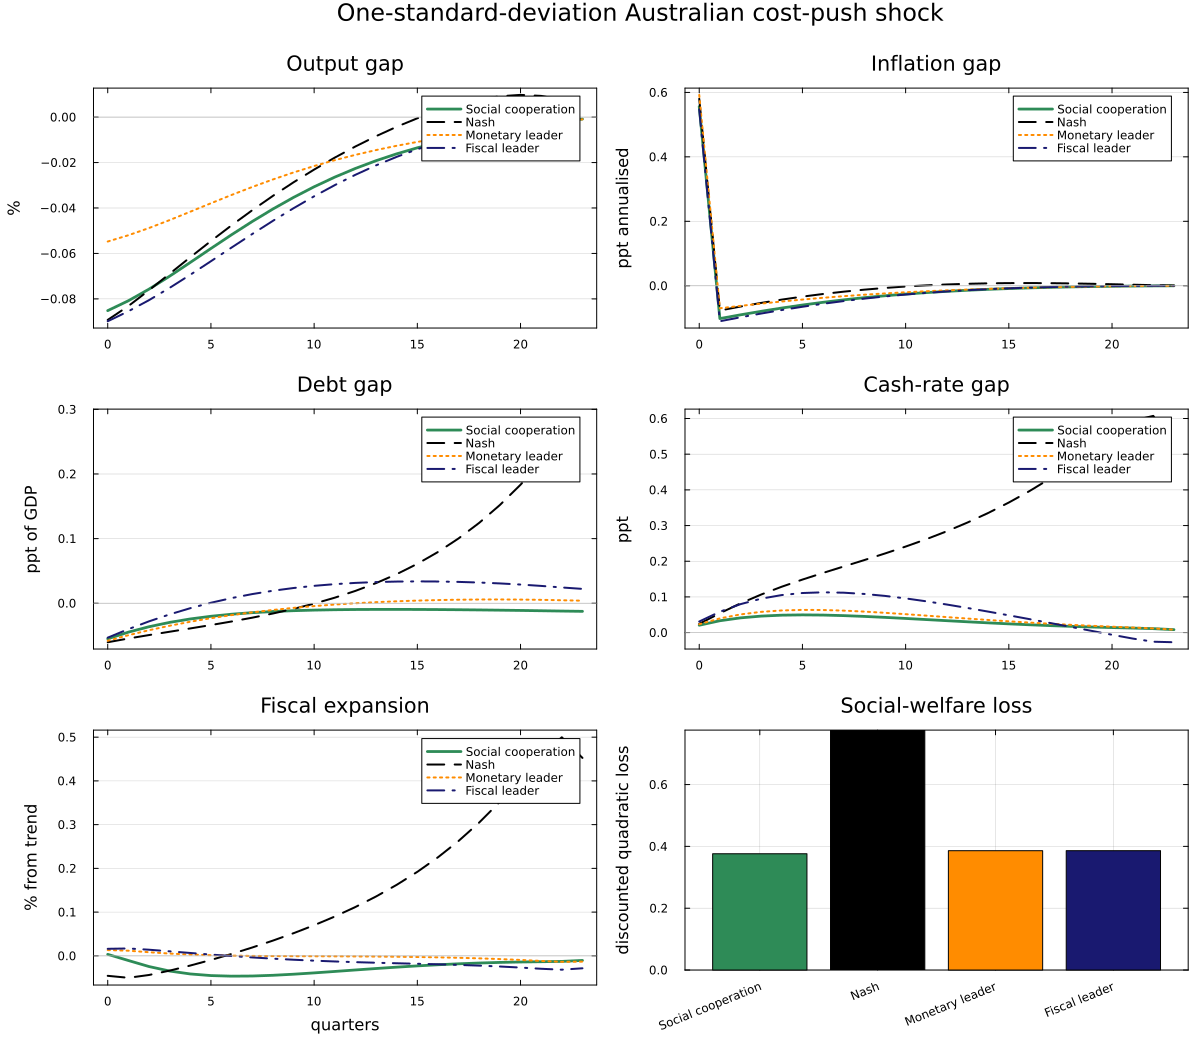
\includegraphics[width=0.94\textwidth]{cost_push_game.png}
\caption{Responses to a cost-push inflation shock.}
\label{fig:supply}
\end{figure}

\subsection{Mandate divergence and the coordination boundary}

At the baseline mandate divergence, the monetary best-response norm is 1.313
and the fiscal norm is 0.742.  The round-trip spectral radius is 0.950, close to
the unit boundary.  This explains why iterated reactions can amplify small
differences and why decentralised policies are so much larger than cooperative
policies.  It does not establish that every element of both reaction matrices
is positive, and it should not be used as a shock-invariant label for the game.

Figures \ref{fig:strategic} and \ref{fig:boundary} show that stronger mandate
divergence and lower instrument costs move the open-loop system toward the
coordination boundary.  The economically important next step is to reproduce
these maps using the eigenvalues of the closed-loop stochastic system and
signed, state-contingent cross-responses.

\begin{figure}[htbp]
\centering
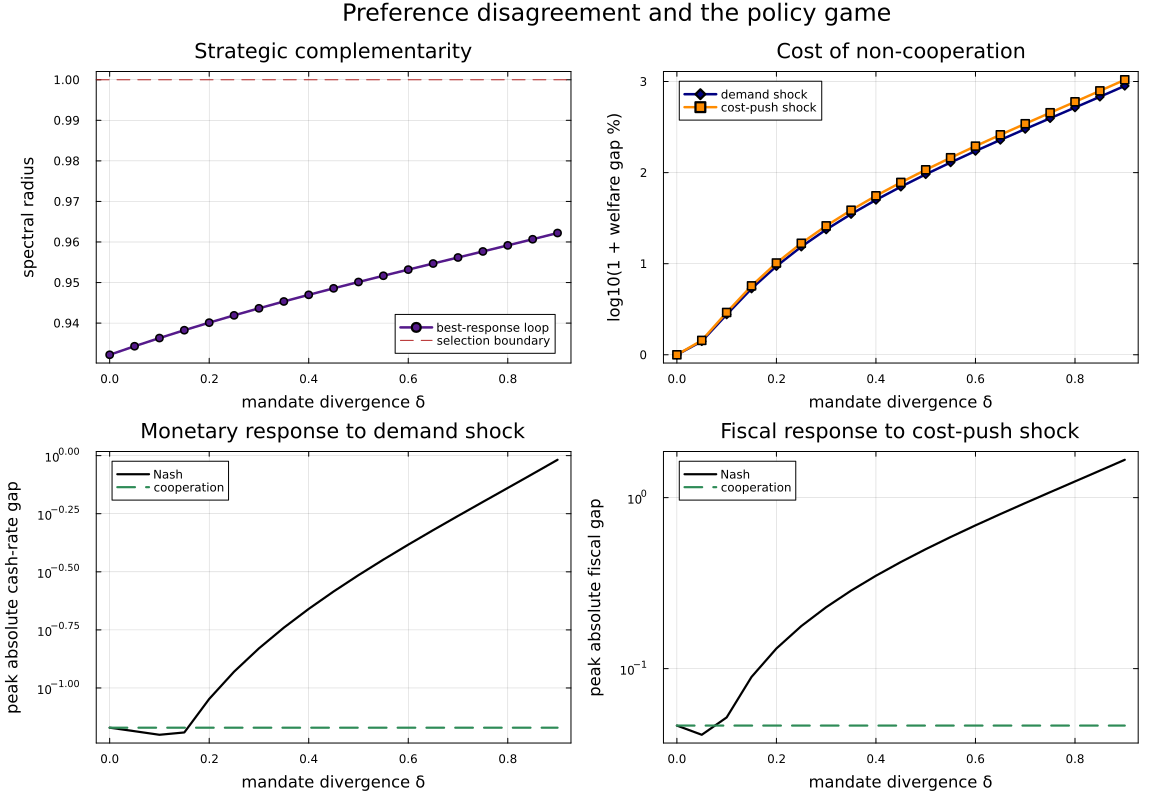
\includegraphics[width=0.94\textwidth]{strategic_complementarity.png}
\caption{Open-loop reaction strength and welfare as agency mandates diverge.}
\label{fig:strategic}
\end{figure}

\begin{figure}[htbp]
\centering
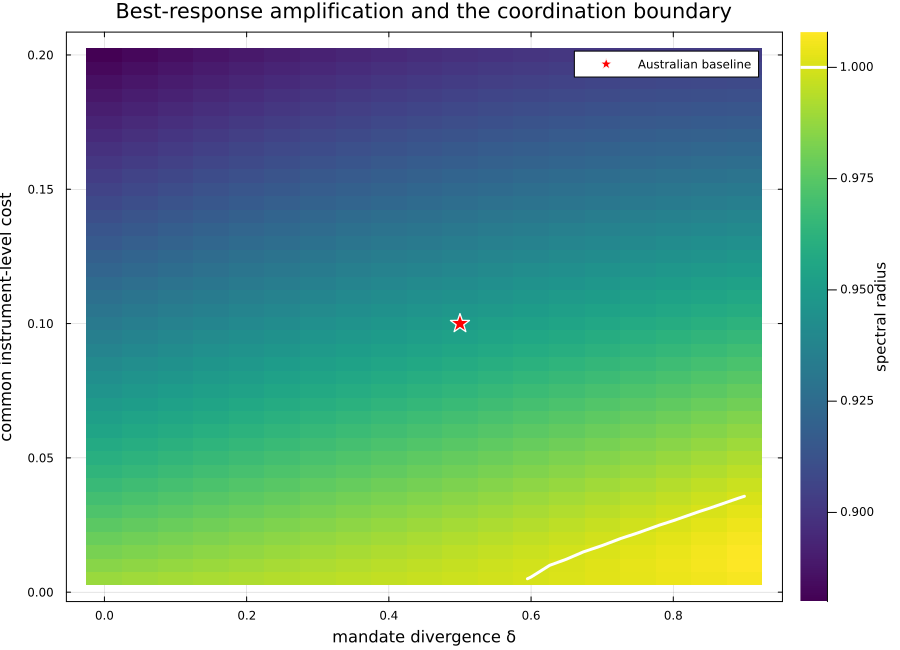
\includegraphics[width=0.82\textwidth]{coordination_boundary.png}
\caption{The open-loop coordination boundary across mandate divergence and
policy-cost calibrations.}
\label{fig:boundary}
\end{figure}

\subsection{Does the model nest fiscal dominance?}

The rule closure nests an active--passive regime comparison in the sense of
\citet{Leeper1991}.  In the monetary-dominance configuration, the interest-rate
rule responds strongly to inflation and fiscal policy stabilises debt.  In the
fiscal-dominance analogue, monetary policy responds weakly and fiscal policy is
less debt responsive.  The latter produces peak inflation of 0.757 versus
0.404 and a peak policy rate of 0.244 versus 0.480 in the monetary-dominance
case.  Figure \ref{fig:dominance} displays the paths.

This is a nesting of the active--passive logic, not a complete fiscal theory of
the price level.  The parsimonious debt equation lets inflation reduce the real
debt gap, which can make the calibrated quadratic social loss lower in the
fiscal-dominance analogue.  A full fiscal-dominance claim requires nominal
government liabilities, a consolidated intertemporal budget constraint,
explicit primary-surplus backing, and equilibrium price-level valuation.  The
current result should therefore be read as a regime diagnostic rather than a
welfare endorsement.

\begin{figure}[htbp]
\centering
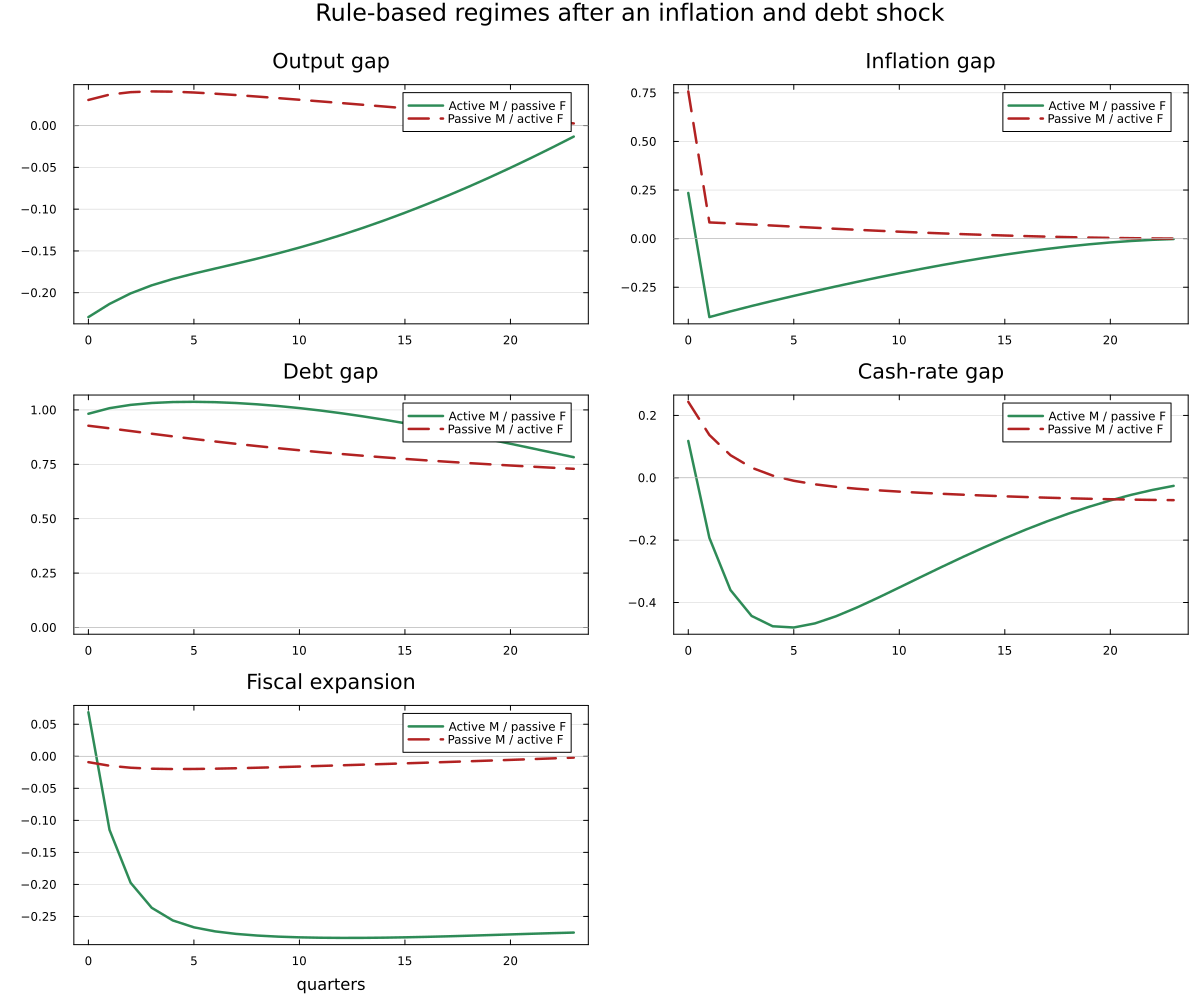
\includegraphics[width=0.94\textwidth]{active_passive_regimes.png}
\caption{Active--passive rule-system comparison.}
\label{fig:dominance}
\end{figure}

\subsection{Recursive Markov-perfect equilibrium}

The recursive feedback Nash calculation converges in 177 coupled Riccati
iterations.  Its closed-loop spectral radius is 0.9383, so the equilibrium is
stable but persistent.  The estimated rules provide direct evidence that
adjustment costs make policy a strategic state.  The monetary rule loads 0.265
on its own lagged instrument and the fiscal rule loads 0.217 on its own lagged
instrument.  When both delegated adjustment coefficients are set to zero,
these two history coefficients are exactly zero.  Current policy therefore
changes not only current demand and inflation, but the marginal cost and
strategic position inherited by future policymakers.

Table \ref{tab:recursive} reports the main recursive results.  The Nash welfare
gap is 0.49 per cent after the demand contraction and 0.06 per cent after the
cost-push shock.  Removing policy inertia increases gross instrument movements
and raises loss.  These gaps are far smaller than in the open-loop experiment.
That finding is important, but it is not evidence that feedback Nash is always
benign: the recursive experiment also changes the private-sector timing from
\eqref{eq:is}--\eqref{eq:pc} to \eqref{eq:ris}--\eqref{eq:rpc}.  A clean
open-loop-versus-feedback comparison requires both concepts to be solved under
the same rational-expectations closure.

\begin{table}[htbp]
\centering
\caption{Recursive equilibrium and delegated adjustment coefficients}
\label{tab:recursive}
\begin{tabular}{lccccc}
\toprule
Regime & $\lambda_M$ & $\lambda_F$ & $\rho(A_{cl})$ & demand loss & supply loss\\
\midrule
Social regulator & --- & --- & 0.9371 & 0.20278 & 0.70775\\
Nash, no inertia & 0 & 0 & 0.9384 & 0.20565 & 0.70964\\
Feedback Nash & 0.050 & 0.040 & 0.9383 & 0.20378 & 0.70816\\
Social institutional design & 0.050 & 0.115 & 0.9382 & 0.20333 & 0.70802\\
\bottomrule
\end{tabular}
\end{table}

\begin{figure}[htbp]
\centering
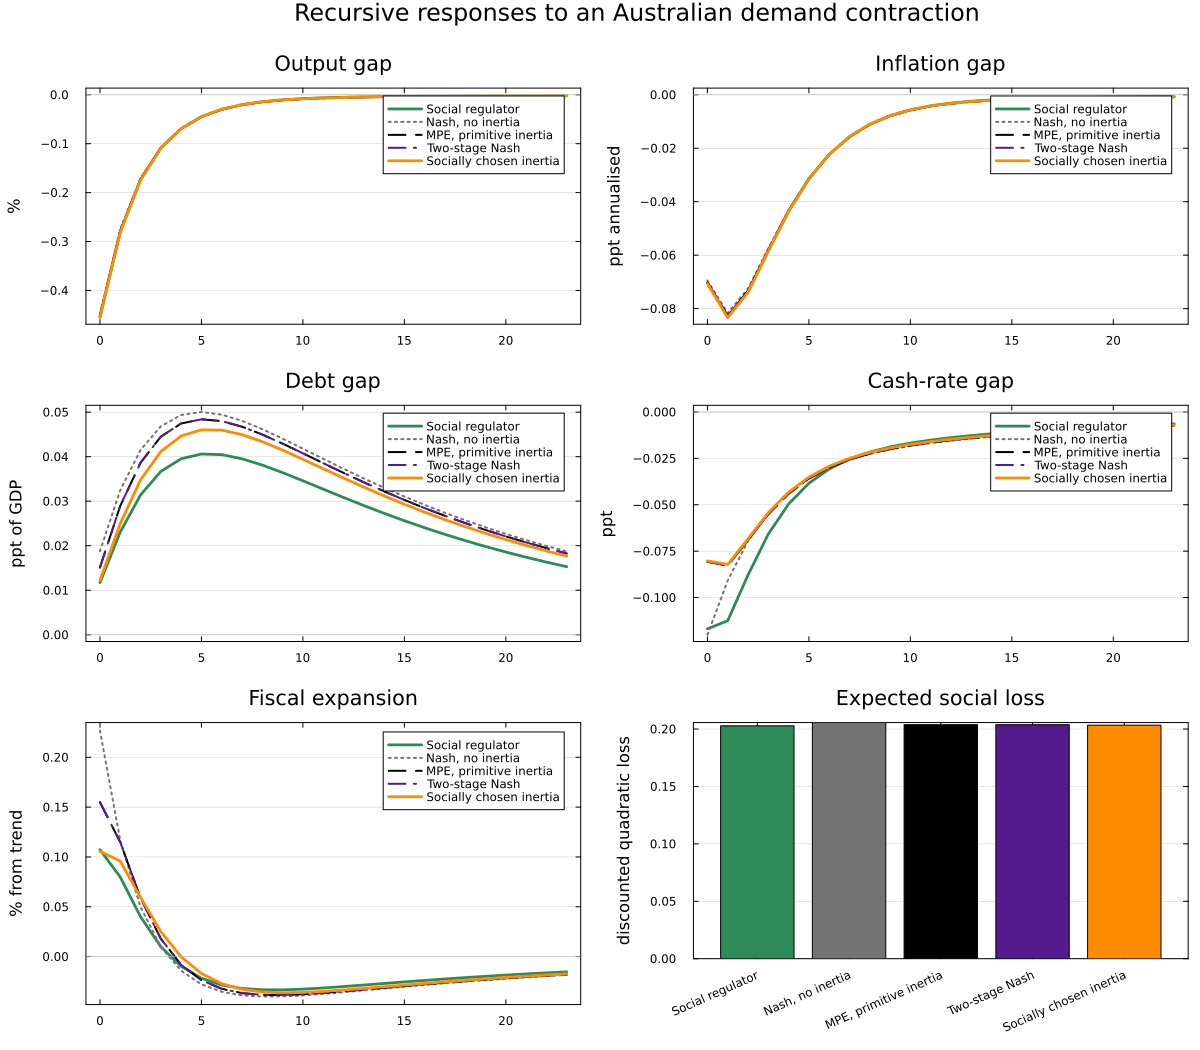
\includegraphics[width=0.98\textwidth]{recursive_demand_game.png}
\caption{Recursive feedback responses to an Australian demand contraction.
The two-stage Nash coincides with the primitive-inertia MPE in the baseline.}
\label{fig:recursive-demand}
\end{figure}

\begin{figure}[htbp]
\centering
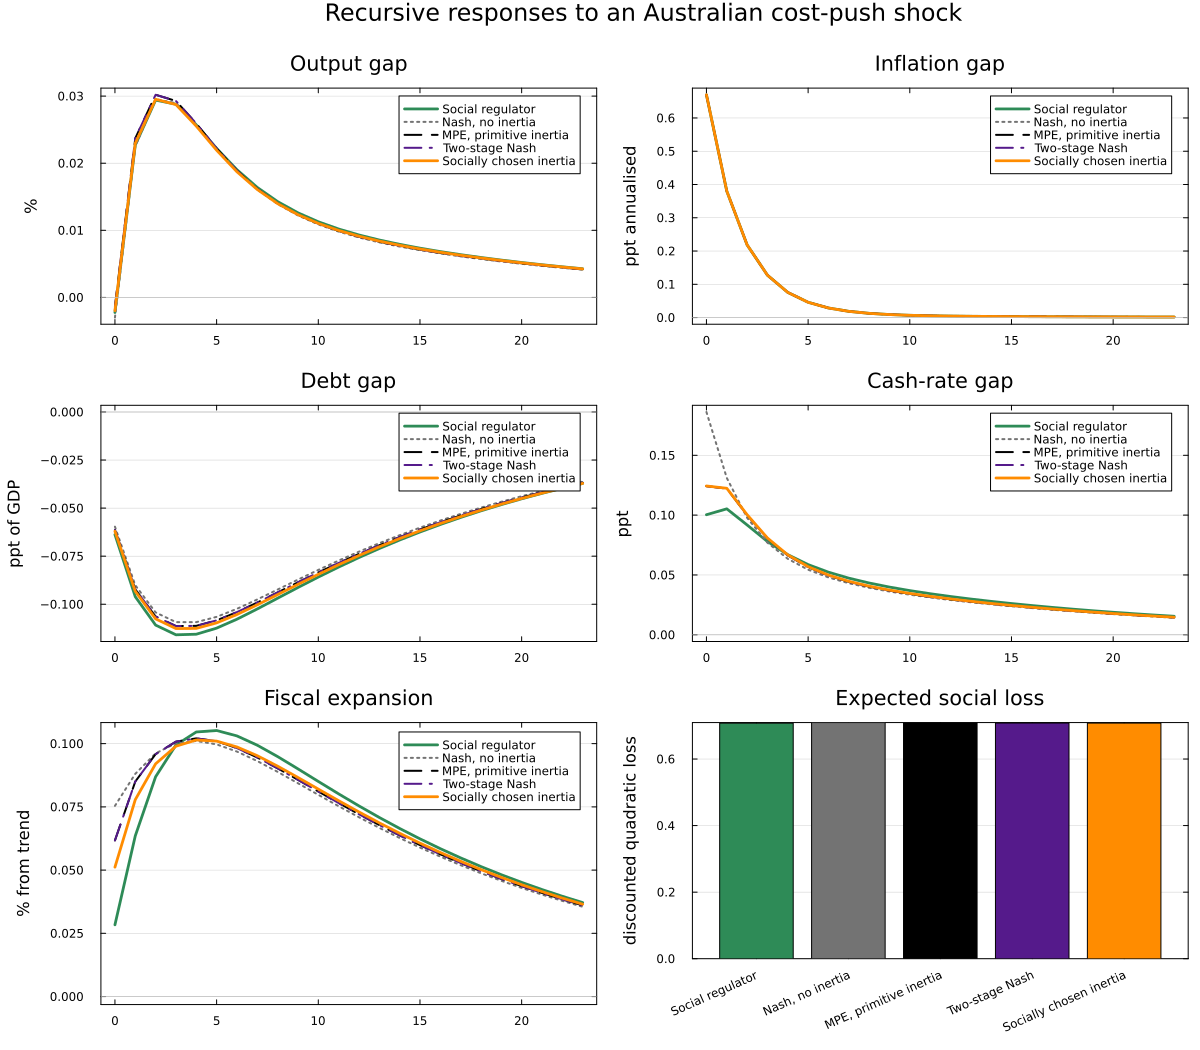
\includegraphics[width=0.98\textwidth]{recursive_cost_push_game.png}
\caption{Recursive feedback responses to an Australian cost-push shock.}
\label{fig:recursive-supply}
\end{figure}

\subsection{The first-stage strategic-investment game}

Figure \ref{fig:commitment} displays the institutional game.  The monetary and
fiscal best-response schedules cross at
$(\lambda_M,\lambda_F)=(0.05,0.04)$, exactly the primitive adjustment weights.
The private stage-one choice therefore does not create an inertia arms race in
this calibration.  This is a substantive negative result: adjustment costs
make current policy an investment in a strategic state, but that fact alone is
not sufficient to generate privately excessive investment in commitment.

The social institutional choice is $(0.05,0.115)$.  Relative to feedback Nash,
it leaves monetary delegation unchanged and almost triples delegated fiscal
inertia.  This reduces the large initial fiscal response to a demand shock from
0.155 to 0.106 and lowers loss in both reported shock experiments.  The
coordination failure in the first stage is therefore under-provision of fiscal
commitment: the fiscal authority does not internalise how a smoother fiscal
rule improves the monetary--fiscal policy mix.  This result is conditional on
the mandate weights, implementation cost, shock distribution, and recursive
timing; the code reports the full objective surface so those assumptions can be
varied rather than hidden.

\begin{figure}[htbp]
\centering
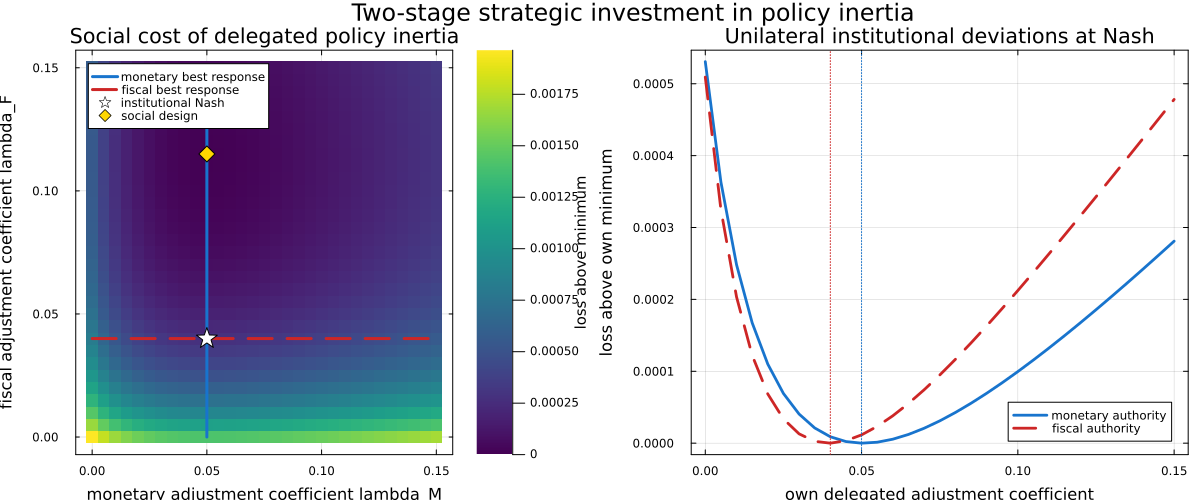
\includegraphics[width=0.98\textwidth]{commitment_game.png}
\caption{The two-stage game in delegated adjustment coefficients.  Lines are
the authorities' discrete best responses; the star is institutional Nash and
the diamond is the social institutional design.}
\label{fig:commitment}
\end{figure}

\section{Is the current approach sufficient?}

The open-loop approach alone is not sufficient for the mechanism in the
motivating draft.  The combined project now supplies both the open-loop
commitment benchmark and a recursive two-stage game.  It demonstrates that
mandate differences can create policy-mix externalities, keeps social
primitives fixed, distinguishes steady state from shocks, and makes lagged
policy a state.  Three boundaries nevertheless remain.

First, a known deterministic shock path eliminates the arrival of new
information.  Second, open-loop paths prevent policies from responding to
off-equilibrium states, whereas debt and lagged instruments are precisely the
states through which strategic commitment operates.  Third, open-loop
leadership conflates leadership with full path commitment; feedback
Stackelberg remains to be solved.  Third, the implemented recursive block is
semi-structural.  It makes timing and persistence transparent, but it does not
yet solve private rational expectations jointly with the feedback rules.
Nominal rigidity makes that remaining omission especially material after a
cost-push shock, because expected future policy affects current inflation and
output.

\begin{table}[htbp]
\centering
\caption{Role of the alternative solution concepts}
\label{tab:concepts}
\small
\begin{tabular}{P{0.22\textwidth}P{0.30\textwidth}P{0.37\textwidth}}
\toprule
Concept & What it identifies & Limitation or role\\
\midrule
Open-loop Nash & Policy-mix externality when complete paths are chosen after a
known shock & Useful commitment benchmark; no reoptimisation after new states\\
Open-loop Stackelberg & Value of internalising the follower's complete-path
reaction & Leadership and full-path commitment are bundled together\\
Feedback/MPE Nash & Discretionary, state-contingent interaction under recurring
shocks & Appropriate main equilibrium for debt and lagged-policy states\\
Feedback Stackelberg & State-contingent strategic leadership & Required to test
whether the two leadership regimes genuinely differ\\
Commitment meta-game & Ex ante choice of adjustment costs, delegation, or rules
& Implemented here; a prisoner's dilemma is possible but does not arise at the baseline\\
\bottomrule
\end{tabular}
\end{table}

\section{What the recursive experiment establishes}

The implemented experiment completes the first three necessary steps:

\begin{enumerate}
  \item It solves the cooperative regulator and stabilising feedback Nash
  equilibrium, verifies convergence and closed-loop stability, and reports the
  full state-contingent rule coefficients.
  \item It shows directly that removing delegated adjustment costs removes the
  own-lag terms from both policy rules.  Policy history is therefore an active
  state rather than a verbal interpretation attached after the calculation.
  \item It solves \eqref{eq:investment} for both authorities and for a social
  institutional designer.  The difference between $(0.05,0.04)$ and
  $(0.05,0.115)$ is the measured first-stage coordination failure.
\end{enumerate}

The next extension should solve the same feedback and open-loop concepts under
one forward-looking rational-expectations block.  That requires finding private
expectation mappings jointly with the coupled policy Riccati equations.  It
should then add feedback Stackelberg equilibria, persistent estimated shock
processes and covariance, and nominal government liabilities for a full fiscal
dominance experiment.  These additions would identify whether the small
recursive welfare gaps are due to feedback discretion itself or to the current
semi-structural timing.

The completed design already lets the steady-state and shock insights reinforce
rather than contradict each other.  The zero-gap deterministic steady state is
a common reference point.  Institutions matter ex ante because they determine
feedback rules used away from that point.  Demand and cost-push shocks activate
different strategic margins, while the commitment stage determines whether
the authorities choose institutions that mitigate those margins.

\section{Conclusion}

Different relative inflation and output weights are sufficient to generate a
substantive monetary--fiscal game once shocks create a macroeconomic trade-off.
They need not create steady-state conflict.  In the Australian calibration,
the no-shock steady state is common to all regimes, but shocks activate the
strategic interaction.  The open-loop benchmark displays a strong offsetting
policy game near its reaction boundary.  The recursive MPE is stable and
history dependent, yet its welfare gaps are modest under the semi-structural
Australian timing.

Most importantly, the two-stage game now distinguishes adjustment costs as
true primitives from adjustment coefficients delegated to future policymakers.
The decentralised institutional equilibrium retains the primitive coefficients;
the social designer instead selects substantially greater fiscal inertia.  The
baseline concern is therefore not excessive strategic investment in commitment
but too little coordinated fiscal commitment.  This negative result disciplines
the theory: strategic-state effects make a commitment game possible, but do not
by themselves guarantee a prisoner's dilemma.  A common forward-looking
private-sector closure and feedback Stackelberg solutions are the remaining
steps needed to determine whether stronger strategic complementarity overturns
that conclusion.

\appendix
\section{Reproducibility}

All calculations and figures are produced by the Julia project accompanying
this paper.  From the project directory, run
\begin{verbatim}
julia --project=. -e "using Pkg; Pkg.instantiate(; update_registry=false)"
julia --project=. run_model.jl
julia --project=. test/runtests.jl
julia --project=. build_tex.jl
\end{verbatim}
The first command installs exact package versions from the manifest.  The model
runner writes calibration primitives, summary tables, the zero-shock audit,
the shock-scaling experiment, recursive policy rules, the complete institutional
objective grid, and all figures to \texttt{output/}.  The final command invokes
the Tectonic binary supplied by Julia's artifact system and creates
\texttt{PAPER.pdf} from this native \LaTeX{} source.

\begin{thebibliography}{99}

\bibitem[Barro and Gordon(1983)]{BarroGordon1983}
Barro, R. J. and Gordon, D. B. (1983).
Rules, discretion and reputation in a model of monetary policy.
\emph{Journal of Monetary Economics}, 12(1), 101--121.

\bibitem[Ba\c{s}ar and Olsder(1999)]{BasarOlsder1999}
Ba\c{s}ar, T. and Olsder, G. J. (1999).
\emph{Dynamic Noncooperative Game Theory}, 2nd ed.
SIAM, Philadelphia.

\bibitem[Dixit and Lambertini(2003)]{DixitLambertini2003}
Dixit, A. and Lambertini, L. (2003).
Interactions of commitment and discretion in monetary and fiscal policies.
\emph{American Economic Review}, 93(5), 1522--1542.

\bibitem[Kydland and Prescott(1977)]{KydlandPrescott1977}
Kydland, F. E. and Prescott, E. C. (1977).
Rules rather than discretion: the inconsistency of optimal plans.
\emph{Journal of Political Economy}, 85(3), 473--491.

\bibitem[Leeper(1991)]{Leeper1991}
Leeper, E. M. (1991).
Equilibria under active and passive monetary and fiscal policies.
\emph{Journal of Monetary Economics}, 27(1), 129--147.

\bibitem[Rogoff(1985)]{Rogoff1985}
Rogoff, K. (1985).
The optimal degree of commitment to an intermediate monetary target.
\emph{Quarterly Journal of Economics}, 100(4), 1169--1189.

\bibitem[Woodford(2003)]{Woodford2003}
Woodford, M. (2003).
\emph{Interest and Prices: Foundations of a Theory of Monetary Policy}.
Princeton University Press.

\bibitem[Australian Government(2023)]{RBAReview2023}
Australian Government (2023).
\emph{An RBA Fit for the Future: Review of the Reserve Bank of Australia}.

\end{thebibliography}

\end{document}
